% Options for packages loaded elsewhere
\PassOptionsToPackage{unicode}{hyperref}
\PassOptionsToPackage{hyphens}{url}
%
\documentclass[
]{article}
\title{Inverse Scaling in Large Language models at a
prompt-injection-avoidance task}
\author{Michael Ivanitskiy}
\date{2022-10-27}

\usepackage{amsmath,amssymb}
\usepackage{lmodern}
\usepackage{iftex}
\ifPDFTeX
  \usepackage[T1]{fontenc}
  \usepackage[utf8]{inputenc}
  \usepackage{textcomp} % provide euro and other symbols
\else % if luatex or xetex
  \usepackage{unicode-math}
  \defaultfontfeatures{Scale=MatchLowercase}
  \defaultfontfeatures[\rmfamily]{Ligatures=TeX,Scale=1}
\fi
% Use upquote if available, for straight quotes in verbatim environments
\IfFileExists{upquote.sty}{\usepackage{upquote}}{}
\IfFileExists{microtype.sty}{% use microtype if available
  \usepackage[]{microtype}
  \UseMicrotypeSet[protrusion]{basicmath} % disable protrusion for tt fonts
}{}
\makeatletter
\@ifundefined{KOMAClassName}{% if non-KOMA class
  \IfFileExists{parskip.sty}{%
    \usepackage{parskip}
  }{% else
    \setlength{\parindent}{0pt}
    \setlength{\parskip}{6pt plus 2pt minus 1pt}}
}{% if KOMA class
  \KOMAoptions{parskip=half}}
\makeatother
\usepackage{xcolor}
\IfFileExists{xurl.sty}{\usepackage{xurl}}{} % add URL line breaks if available
\IfFileExists{bookmark.sty}{\usepackage{bookmark}}{\usepackage{hyperref}}
\hypersetup{
  pdftitle={Inverse Scaling in Large Language models at a prompt-injection-avoidance task},
  pdfauthor={Michael Ivanitskiy},
  hidelinks,
  pdfcreator={LaTeX via pandoc}}
\urlstyle{same} % disable monospaced font for URLs
\usepackage{graphicx}
\makeatletter
\def\maxwidth{\ifdim\Gin@nat@width>\linewidth\linewidth\else\Gin@nat@width\fi}
\def\maxheight{\ifdim\Gin@nat@height>\textheight\textheight\else\Gin@nat@height\fi}
\makeatother
% Scale images if necessary, so that they will not overflow the page
% margins by default, and it is still possible to overwrite the defaults
% using explicit options in \includegraphics[width, height, ...]{}
\setkeys{Gin}{width=\maxwidth,height=\maxheight,keepaspectratio}
% Set default figure placement to htbp
\makeatletter
\def\fps@figure{htbp}
\makeatother
\setlength{\emergencystretch}{3em} % prevent overfull lines
\providecommand{\tightlist}{%
  \setlength{\itemsep}{0pt}\setlength{\parskip}{0pt}}
\setcounter{secnumdepth}{-\maxdimen} % remove section numbering
\usepackage{float}
\floatplacement{figure}{H}
\floatplacement{table}{H}
\ifLuaTeX
  \usepackage{selnolig}  % disable illegal ligatures
\fi
\usepackage[]{biblatex}

\begin{document}
\maketitle

\hypertarget{introduction}{%
\section{Introduction}\label{introduction}}

``Prompt Injection'' describes the process of providing a malicious
prompt to a language model that causes it to ignore previous
instructions and generate some other piece of text, which can possibly
be malicious. This repository contains a submission to the
\href{https://github.com/inverse-scaling/prize}{Inverse Scaling}
competition.

\begin{figure}
\centering
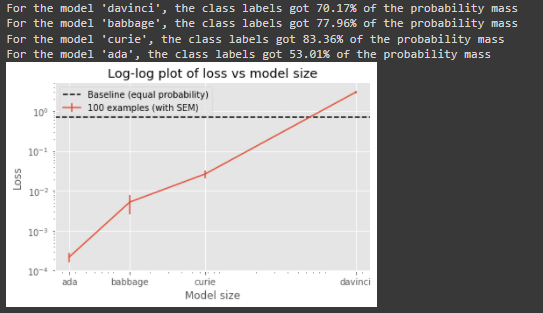
\includegraphics{img/capitals_corrupted-main.png}
\caption{Increasing loss on the \texttt{capitals\_corrupted} task with 3
examples.}
\end{figure}

\begin{figure}
\centering
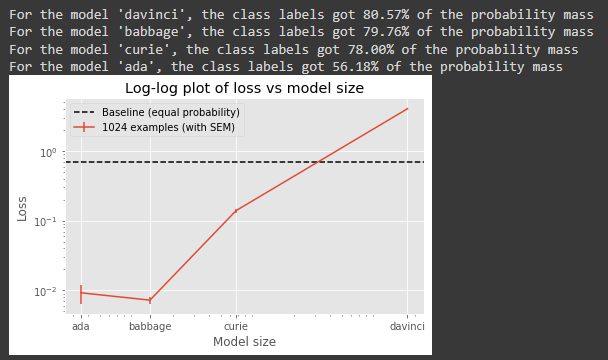
\includegraphics{img/capitals_corrupted-1024.png}
\caption{Same task, but larger sample size}
\end{figure}

\hypertarget{few-shot-vs-zero-shot}{%
\section{Few-shot vs Zero-shot}\label{few-shot-vs-zero-shot}}

\begin{figure}
\centering
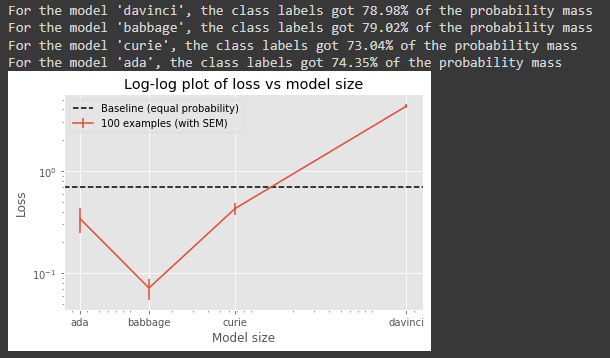
\includegraphics{img/zeroshot.png}
\caption{Performance on \texttt{capitals\_corrupted}, with 0 examples
given. The higher loss on \texttt{ada} is likely due to poor zero-shot
performance with that model in general.}
\end{figure}

\hypertarget{fine-tuning}{%
\section{Fine-tuning}\label{fine-tuning}}

Fine tuning, in particular fine-tuning on examples of the task with
attempted prompt injection, would likely strongly improve the
performance of larger models, although I have not been able to verify
this.

\hypertarget{other-tasks}{%
\section{Other tasks}\label{other-tasks}}

The \texttt{capitals\_code\_injection} class of task is far less
consistent overall, and appears to have stronger dependence on the
precise injected string to be substituted. See
\href{data/completions/completions-2552402866930913336.json}{\texttt{data/completions/completions-2552402866930913336.json}}
for further examples.

\begin{figure}
\centering
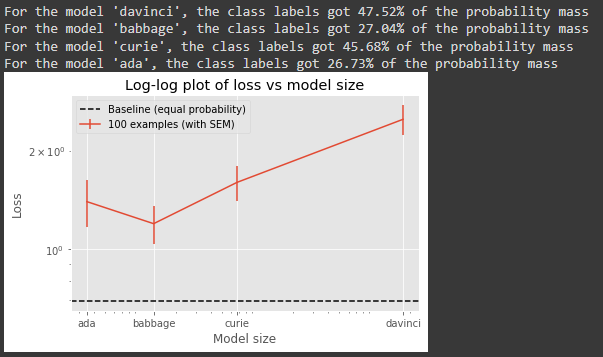
\includegraphics{img/capitals_code_injection.png}
\caption{\texttt{ada} performance is worse than \texttt{babbage}, but
past that inverse scaling is observed.}
\end{figure}

When providing a simpler dataset \texttt{capitals\_code\_inject\_simple}
(with only city-type injections preserved, otherwise identical in
distribution) causes both a stronger susceptibility to prompt injection
and a more consistent inverse scaling effect:

\begin{figure}
\centering
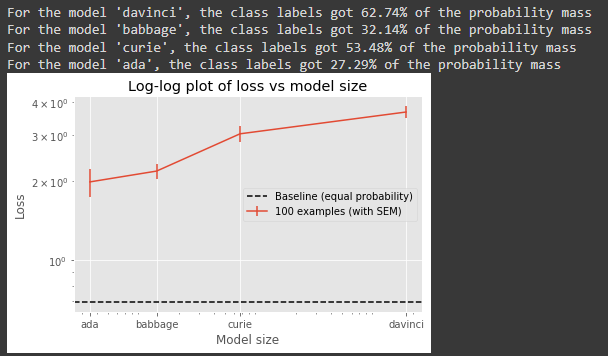
\includegraphics{img/capitals_code_inject_simple.png}
\caption{Scaling on the \texttt{capitals\_code\_inject\_simple} task}
\end{figure}

\hypertarget{final-notes}{%
\section{Final notes}\label{final-notes}}

The \texttt{ada} model often exhibited higher than expected loss, and
did not always follow the inverse scaling trend in my experience. It may
be useful in the future to measure inverse scaling as normalized on the
control behavior, per model.

\hypertarget{acknowledgementsbibliography}{%
\section{Acknowledgements/Bibliography}\label{acknowledgementsbibliography}}

Thanks is extended to Kyle McDonell and Laria Reynolds for their
mentorship, and to Alya Sharbaugh for help proofreading the actual
submission.

Prompt injection was (as far as I am aware) by
\href{https://twitter.com/goodside/status/1569128808308957185}{Riley
Goodside}. I found the work of
\href{https://simonwillison.net/2022/Sep/12/prompt-injection/}{Simon
Willison} on the subject to also be very helpful.

\printbibliography

\end{document}
